\documentclass[a4paper]{amsart}

\usepackage{color}
\usepackage[colorlinks=true, citecolor=red]{hyperref}  %needs to come before amsrefs package to work with \cite{}*{}
\usepackage{amssymb,latexsym}
\usepackage[alphabetic]{amsrefs}
\usepackage[mathscr]{eucal}
\usepackage{pdfsync}
\usepackage{graphicx}
\usepackage{epstopdf}
\DeclareGraphicsRule{.tif}{png}{.png}{`convert #1 `dirname #1`/`basename #1 .tif`.png}
\usepackage[all]{xy}
\usepackage{titletoc}
%\usepackage{txfonts}   %  \fint  for integral average

%\usepackage{showkeys}  %options notref  notcite 

%\input{rgb.tex}

%\textcolor{DarkRed}{text in DarkRed}


\CompileMatrices

\theoremstyle{plain}
\newtheorem{theorem}{Theorem}[section]
\newtheorem{lemma}[theorem]{Lemma}
\newtheorem{proposition}[theorem]{Proposition}
\newtheorem{corollary}[theorem]{Corollary}

\theoremstyle{definition}
\newtheorem{definition}[theorem]{Definition}%[section]


\theoremstyle{remark}
\newtheorem{defn}[theorem]{Definition} 
\newtheorem{example}[theorem]{Example}
\newtheorem{remark}[theorem]{Remark}
\newtheorem{discussion}[theorem]{Discussion}

%\numberwithin{equation}{section}

%\newcommand{\abs}[1]{\lvert#1\rvert}

\DeclareMathOperator{\Lip}{Lip}
\DeclareMathOperator{\dist}{dist}
\DeclareMathOperator{\expected}{\mathbb{E}}
\DeclareMathOperator{\prb}{Prob}
\DeclareMathOperator{\spt}{spt}
\DeclareMathOperator{\lap}{\Delta}
\DeclareMathOperator{\Tr}{Tr}

\raggedbottom

%\addtolength{\textwidth}{2cm}
%\addtolength{\oddsidemargin}{-1cm}
%\addtolength{\evensidemargin}{-1cm} 
%\addtolength{\topmargin}{-1cm} 
%\addtolength{\textheight}{2cm}

 
%%% BEGIN DOCUMENT
\begin{document}

\title{Linear Programming and Duality}  
\author{John E.\ Hutchinson}
\date{\today}

\begin{abstract} 
This includes a simple geometrically motivated  proof of Farkas' Lemma, and of the LP duality theorem as a consequence, without using the simplex algorithm. See Theorems~\ref{ThmLP} and~\ref{ThmFar}.  There are no new ideas, but the argument is shorter and clearer than what I have seen elsewhere.

The main source is \cite{BT}*{Chapter 4}.


\end{abstract}

\maketitle

\tableofcontents


%%%%%%%%%%%%%%%%%%%%%%%%%%%%%%%%
%%%%%%%%%%%%%%%%%%%%%%%%%%%%%%%%
%%%%%%%%%%%%%%%%%%%%%%%%%%%%%%%%
%%%%%%%%%%%%%%%%%%%%%%%%%%%%%%%%
\section{\textbf{Outline of Main Theorem and Proof}}  

\noindent \emph{This section provides enough information to motivate and construct the proof.}

\bigskip
\emph{See Figure~\ref{poly}}. 
Consider the primal LP problem in standard form:
\begin{equation} \label{primal}
\begin{aligned}
\text{minimise} \quad & cx \\
\text{subject to} \quad & Ax \geq b ,
\end{aligned}
\end{equation} 
where $ c \in (\mathbb{R}^n )^* $, $ x \in \mathbb{R}^n $, $ A $ is an $ m\times n $ matrix, and $ b \in \mathbb{R}^m$.  
 
The \emph{dual} problem is   
\begin{equation} \label{dual}
\begin{aligned}
\text{maximise} \quad & yb \\
\text{subject to} \quad & yA=c,\ y \geq 0,
\end{aligned}
\end{equation} 
 where $ y \in (\mathbb{R}^m )^*$.
 
\begin{theorem}\mbox{}
\begin{enumerate}
\item For any $ x $ and $ y $ that are primal and dual feasible respectively, $ yb \leq cx $.
\item If there is a primal solution $ x^* $ then there is a dual solution $ y^* $ which is a \emph{positive} linear combination of the inward normals for the active constraints at $ x^* $.  That is, $ y^* $   is a \emph{positive} linear combination of those rows $ A_i $ of $ A $ such that $ A_i x^* = b_i $.
\item If $ x^* $ and $ y^* $   are primal and dual feasible respectively, then $ y^*b  = cx^* $.
\end{enumerate} 
\end{theorem} 

\begin{proof} \mbox{}
\begin{enumerate}

\item If $ x $ and $ y $   are primal and dual feasible respectively then $ yb \leq yAx = cx $.
\medskip

\item $ x^* $ is a solution of the new primal problem obtained by removing those constraints inactive at $ x^* $. This is clear from Figure~\ref{feasible}, which also motivates the proof. 

Let $ I \subset \{1,\dots, m\} $ denote the active constraints at $ x^* $.

Then the polyhedral cone
\[
 \mathcal{C} = \{x : A_i x  \geq b_i\  \forall i\in I \}  
 \]
is the feasible region for the new primal problem. 

Without loss of generality $ x^* = 0 $. Hence  
\[  b_i = 0   \text{ for }  i\in I ,\quad 
 \mathcal{C} = \{ x : A_ix \geq 0\ \forall i\in I \}  , \quad    cx\geq 0 \text{ for } x \in \mathcal{C}  .
 \]

By definition,   $ c $ is in the dual cone $ \mathcal{C} ^* $.
But by Farkas' Lemma
\[
 \mathcal{C} ^* =   \sum_i \big\{ y_iA_i :   i \in I,\ y_i\geq 0   \big\}
 \]
We just need ``$ \subset $'' in the previous line, and this is proved using a simple separating hyperplane argument applied to the cone on the right side of the equality.  See the proof of Farkas' Lemma.  Or see the ``gravitational'' explanation  in Remark~\ref{grav}.

\medskip
By setting  $ y_i=0 $ in the previous equality  if $ i \notin I $, it follows for some $ y^* $ that 
\[
c = y^* A, \quad y^* \geq 0, \quad y_i^*=0 \text{ if } i \notin I .
\]
Hence
\[  
cx^* = y^*Ax^* = y^* b,
\]
For the last inequality use $ A_ix^*=b_i $ if $ i \in I $,  and   $ y_i^*=0 $ if $ i \notin I $. 

\medskip
\item It follows that 
\[
cx^* = y^* b 
\]
for \emph{any} solutions $ x^* $ and $ y^* $ of the primal and dual problems.
\end{enumerate} 

\end{proof}


%%%%%%%%%%%%%%%%%%%%%%%%%%%%%%%%
%%%%%%%%%%%%%%%%%%%%%%%%%%%%%%%%
%%%%%%%%%%%%%%%%%%%%%%%%%%%%%%%%
%%%%%%%%%%%%%%%%%%%%%%%%%%%%%%%%
\section{\textbf{Preliminaries}} 

\noindent \emph{This section is just basic notation.} 
 
 
\emph{Points}  $ x \in \mathbb{R}^n $ are represented by \emph{column} vectors 
$ x = \begin{bmatrix}  x_1 \\ \vdots \\ x_n \end{bmatrix} $. 

For typographic reasons we write $ x = (x_1,\dots x_n) $.  Note   ``$ ( , ) $''  instead of ``$ [ , ] $''.

For multiplicative purposes we regard $ x $ as a $ n \times 1 $ matrix.
 
\bigskip
\emph{Linear functionals} $ c \in ( \mathbb{R}^n )^* $ are represented by row vectors $ c = [c_1  \dots c_n ] $.  
The action on $ x $ is given by matrix multiplication 
\[
cx = \sum_i c_i x_i . 
\]

Geometrically, if $ c $ is non zero then $ c $ is represented by a family of parallel hyperplanes, one for each level set of $ c $. See Figure~\ref{hyper}.


\begin{figure}[htbp] %  figure placement: here, top, bottom, or page
   \centering
   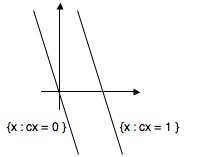
\includegraphics[width=2in]{hyperplane.jpg} 
   \caption{Two level sets corresponding to a linear functional $ c $.}
   \label{hyper}
\end{figure}

Sometimes we think of $ c $ as a ``cost'' vector and $ cx $ as the cost of the ``commodity bundle'' $ x $.

\bigskip
\emph{Order Relation.}  By $ x \geq 0 $ we mean $ x_i\geq 0 $ for all $ i $.  Similarly for $ c \geq 0 $, etc.

\bigskip
\emph{Feasible region.}  Suppose $ A $ is a given $ m\times n $ matrix.  The rows are denoted $ A_i $.  Consider the polyhedral region $ R $, possibly unbounded, given by the constraints
\[
R = \{ x : Ax \geq b \} = \{ x : A_i x \geq b_i \ \forall i = 1,\dots , m \},
\]
where $ b \in \mathbb{R}^m $ (see Figure~\ref{poly}).  We say $ R $ is the \emph{feasible} region  and elements $ x\in R $ are \emph{feasible}.  We can also consider constraints of the form $ A_i x \leq b_i $ or $   A_i x = b_i $


\begin{figure}[htbp] %  figure placement: here, top, bottom, or page
   \centering
   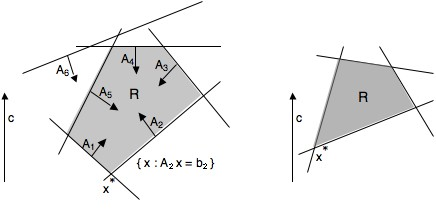
\includegraphics[width=3.5in]{poly.jpg} 
   \caption{The feasible region $ R $ consists of those $ x $ satisfying $ A_i x \geq b_i $ for all $ i $.  The normal vectors $ A_i $ point   ``into'' $ R $, even for $ A_6 $.  The constraints $  A_1 x \geq b_1 $ and $ A_2 x \geq b_2$ are active at $ x^*$, and the other constraints are inactive.}
   \label{poly}
\end{figure}


The constraint $ A_i \geq b_i $ is \emph{active} at $ x $ if $ A_i x = b_i $, and otherwise the constraint is \emph{inactive}.



%%%%%%%%%%%%%%%%%%%%%%%%%%%%%%%%
%%%%%%%%%%%%%%%%%%%%%%%%%%%%%%%%
%%%%%%%%%%%%%%%%%%%%%%%%%%%%%%%%
%%%%%%%%%%%%%%%%%%%%%%%%%%%%%%%%
\section{\textbf{Farkas' Lemma}}   

\noindent \emph{This is a basic result.}

 \begin{remark}[Motivation]  \label{grav} See Figure~\ref{cone}.
 
 \begin{figure}[htbp] %  figure placement: here, top, bottom, or page
   \centering
   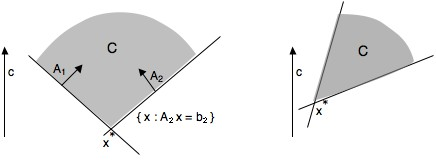
\includegraphics[width=3.5in]{cone.jpg} 
   \caption{In both cases the hypotheses of Farkas' lemma are satisfied.  Note that in the second figure $ c \not\in \mathcal{C} $ when the base of $ c $ is placed at $ x^* $.}
      \label{cone}
\end{figure}


Think of  $ c $ as both an element of $ \mathbb{R}^n $  and an element of the dual $ (\mathbb{R}^n )^*$, in which case $ c \cdot x $ corresponds to  $ c \cdot x $. 
 
 
  Suppose $ \mathcal{C} $ is a \emph{polyhedral cone}   in $ \mathbb{R}^n $ with vertex $ x^* $  and is given by the intersection of half spaces $ \{x : A_i x \geq b_i \}$  for $ i = 1,\dots, m $.  By the statement ``\,$ x^*$ 
   is (a) vertex
   \footnote{The ``$ \mbox{}^* $ '' is conventional for minimisers.}
    of $ \mathcal{C} $\,'' is meant  that   $ A_i x^* = b_i  $  for all $ i  $, i.e.\ $ Ax^* = b$, i.e.\ \emph{all constraints are  \underline{active} at $ x ^* $}.  

Suppose $ \mathcal{C} $ is a subset of the half space through $ x^* $ determined by the normal vector $ c $.  Then Farkas' Lemma says $ c $   is a linear combination of the inward pointing normals $ A_i $ with \emph{non negative} coefficients.

For motivation, suppose gravity acts in the direction $ -c $ and consider a small ball $ B $ inside the cone $ \mathcal{C}  $. The ball will be in equilibrium just above the vertex $ x^ * $, where the gravitational force is exactly balanced by (inward) normal forces from each of the hyperplanes in contact with $ B $.  That is $ c = \sum y_i A_i^t $ with $ y_i \geq 0 $.
 \hfill $\square$  \end{remark} 
 
 %%%%%%%%%%%%%%%

\begin{remark}[Dual of a Polyhedral Cone]  \label{rmkdual} If $ \mathcal{C} $ is a cone with vertex at the origin, the \emph{dual cone} $ \mathcal{C} ^* $ in $ \mathbb{R}^n $ is defined by
\[
\mathcal{C} ^* = \{ z\in \mathbb{R}^n  : z \cdot x \geq 0\ \forall x \in \mathcal{C}  \}.
\]
See Figure~\ref{figdual}.  Equivalently, working in $ (\mathbb{R}^n)^* $, the dual of $ \mathcal{C} $ is
\[
\mathcal{C} ^* = \{ z\in (\mathbb{R}^n)^*  : z  x \geq 0\ \forall x \in \mathcal{C}  \}.
\]

Note $ \mathcal{C} = \mathcal{C}^{**} $.




\begin{figure}[htbp] %  figure placement: here, top, bottom, or page
   \centering
   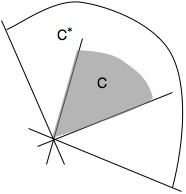
\includegraphics[width=1.3in]{dual.jpg} 
   \caption{A cone $ C $ and its dual $ C^* $.  Note $ C^{**} = C $.}
   \label{figdual}
\end{figure}

Farkas' Lemma essentially says  for a polyhedral cone $ \mathcal{C} = \{ x : Ax \geq 0 \} $  that the dual cone is given by
\[
\mathcal{C} ^* = \left\{ \sum_i y_i  A_i^t : y_i \geq 0 \right\}.
\]
(We take the transpose of the row vectors $ A_i $ so as  to obtain column vectors in $ \mathbb{R}^n $.)

Notationally, it is clearest to prove the equivalent version in  $ (\mathbb{R}^n)^* $:
\[
\mathcal{C} ^* = \{ yA : y \geq 0 \}.
\]
The inclusion ``$ \subset $'' was shown in the proof of Farkas' Lemma.  The inclusion ``$ \supset $'' is by the definitions:  Consider $ yA $ where $ y \geq 0 $.  If $ x \in \mathcal{C} $, i.e.\  $ Ax \geq 0 $, then  immediately it follows  $ yAx \geq 0$.   Hence $ yA \in \mathcal{C} ^* $.
\hfill $\square$  \end{remark}
 
 


\begin{theorem}[Farkas' Lemma]  \label{ThmFar} Let $ \mathcal{C} $ be the cone $  \{ x : Ax \geq b \}\subset \mathbb{R}^n   $ where $ A $ is $ m \times n $ and the vertex $ x^* $ satisfies  $ Ax^* = b  $ . 
   Suppose $ c \in ( \mathbb{R}^n )^* $ and $c x^* \leq cx $ for  all $ x \in  \mathcal{C}$.  Then there exists $ y \in   (\mathbb{R}^m)^*   $ with
   \[
   c = \sum_i y_i A_i = yA , \quad y \geq 0 .
   \]
   (See Figure \ref{cone}.)
\end{theorem} 

\begin{proof}
 By translating $ x^* $ to the origin we may assume $ x^* = 0 \in \mathbb{R}^n $. Hence  $ b = 0 \in \mathbb{R}^m $, 
$\mathcal{C} = \{ x : Ax \geq 0 \} $, and $ cx\geq 0 $ for $ x \in \mathcal{C} $.

We W.T.S.
 that   
 $ c \in   \{ yA : y \geq 0 \} =:\widetilde{\mathcal{C}} $.
 \footnote{In fact $  \widetilde{\mathcal{C} }$  is precisely the dual   of   $ \mathcal{C} $, see Remark~\ref{rmkdual}.}

  
Assume $ c \notin :\widetilde{\mathcal{C}} $. 

Since $ \widetilde{\mathcal{C}}$ is a convex set (in fact cone) containing $ 0 $ there exists a closed half space containing $ \widetilde{\mathcal{C}}$ but not containing $ c $. If the half space is given by $ z\in \mathbb{R}^n  $ then 
\[  cz < 0, \quad y \geq 0 \Longrightarrow yAz \geq 0 .\]

Since $ cz < 0 $, $ z \notin \mathcal{C} $. 

From the implication, $ Az \geq 0 $, i.e.\  $ z \in \mathcal{C} $.  

This contradiction completes the proof.
\end{proof} 




 
 %%%%%%%%%%%%%%%%%%%%
 \begin{remark} The vector $ y^* $ is not necessarily unique.  For example, in $ \mathbb{R}^3 $, suppose the ball in Remark~\ref{cone}  is supported by 4 or more walls.
\hfill $\square$  \end{remark}  
 
 
 
 
%%%%%%%%%%%%%%%%%%%%%%%%%%%%%%%%
%%%%%%%%%%%%%%%%%%%%%%%%%%%%%%%%
%%%%%%%%%%%%%%%%%%%%%%%%%%%%%%%%
%%%%%%%%%%%%%%%%%%%%%%%%%%%%%%%%
\section{\textbf{Duality in Linear Programming}}   

\noindent \emph{This is the basic linear programming result.} 



 \bigskip 
Consider the linear programming [LP] problem in standard form:
\begin{equation} \label{primal}
\begin{aligned}
\text{minimise} \quad & cx \\
\text{subject to} \quad & Ax \geq b ,
\end{aligned}
\end{equation} 
where $ c \in (\mathbb{R}^n )^* $, $ x \in \mathbb{R}^n $, $ A $ is an $ m\times n $ matrix, and $ b \in \mathbb{R}^m$.  
 
 By straightforward manipulations, linear maximisation problems, linear constraints of the form ``$ \leq $'', and linear equality constraints, are also included. 
 
Problem \ref{primal} is called the \emph{primal problem}.  The \emph{dual} problem is then 
\begin{equation} \label{dual}
\begin{aligned}
\text{maximise} \quad & yb \\
\text{subject to} \quad & yA=c,\ y \geq 0,
\end{aligned}
\end{equation} 
 where $ y \in (\mathbb{R}^m )^*$.
 
 In the following discussion will see one way in which the dual problem arises naturally.
 
 \begin{theorem}[LP Duality Theorem] \label{ThmLP} \mbox{}
 \begin{enumerate}

\item \emph{Weak Duality:}  If $ x $ is feasible for the primal problem and $ y $ for the dual problem then
 \[ yb \leq cx .\]
 \item \emph{Existence of a Solution of the Dual Problem:}  If $ x^* $ is a solution of the primal problem and $ y^* $ is obtained by applying Farkas' Lemma to those rows of $ A $ which are active for $ x^* $, then  $ y^* $ is a solution of the dual problem.
 
 \item \emph{Strong Duality:}  If $ y^* $ is \emph{any} solution of the dual problem then 
 \[   y^*b  = cx^* .\]
\end{enumerate}
\end{theorem}

\begin{proof} 
 \begin{enumerate}

\item We have
\begin{align*}
yb &\leq yAx \quad \text{since } y\geq 0, \  b \leq Ax \\
  & = cx   \quad \text{since }  yA = c .
  \end{align*} 
  \bigskip 
  
  \item By translation assume $ x^* = 0 $. This will change $ b $ but not $ A $.
  
  Suppose $ A_i $ is active at $ 0 $ for $ i \in I $ and inactive for $ i \notin I $.  Since $ 0 $ is feasible, 
  \[
  i\in I \Longrightarrow b_i =0, \quad i \notin I \Longrightarrow b_i < 0 .
  \]
  
  Let 
  \[
   \mathcal{C} = \{ x \in \mathbb{R}^n : A_i x \geq 0 \ \forall i \in I \}.
   \]
 be the cone generated by the constraints active at $ 0 $. 
  
  We \emph{claim} that if $ x \in \mathcal{C}$ then $ \epsilon x $ is feasible for the primal problem for sufficiently small $ \epsilon > 0 $.  See Figure~\ref{feasible}. 
  
 \begin{figure}[htbp] %  figure placement: here, top, bottom, or page
    \centering
    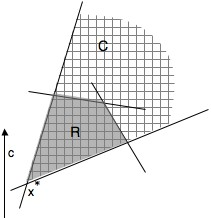
\includegraphics[width=1.6in]{feasible.jpg} 
    \caption{$ C $ is the cone generated by the active constraints at $ x^*  $ and $ R $ is the feasible region for the LP problem.  If $ x $ is in the cone given by the active constraints at $ x^* $ then $ \epsilon x $ is feasible for sufficiently small $ \epsilon > 0 $.}
    \label{feasible}
 \end{figure} 
  
If $ i \in I $ then  $   A_i x \geq 0 $ and so $ A_i (\epsilon x) \geq 0=b_i $.
  
If $ i \notin I $ then $ b_i < 0 $ and so $ A_i (\epsilon x) \geq b_i $ if $ \epsilon >0 $ is sufficiently small.  
  
This establishes the \emph{claim}.

\medskip
Since $ x^*=0 $ minimises the primal problem and $ \epsilon x $ is is feasible,
\begin{align*} 
 c(\epsilon x) \geq c x^* &= 0 \\
 \text{and so} \quad cx &\geq 0 \text{ if } x \in \mathcal{C} .
 \end{align*} 

Now apply Farkas' Lemma to deduce    
   \[
   c  = \sum_{i\in I} y_i^*A_i , \quad \text{where } y_i^* \geq 0 .
   \]
It follows that
\begin{equation} \label{seq} 
cx^*  = \sum_{i\in I}  y_i^* A_i x^* = \sum_{i\in I} y_i^* b_i = y^*b ,
\end{equation} 
where we define $ y_i^* = 0 $ for $ i\notin I $.
This, together with weak duality, implies $ y^* $ maximises the dual problem.
\bigskip 

\item It follows from weak duality and~\eqref{seq} that 
\[
cx^* = y^* b 
\]
for \emph{any} solutions $ x^* $ and $ y^* $ of the primal and dual problems respectively.
\end{enumerate}
\end{proof}
 
 

%%%%%%%%%%%%%%%%%%%%%%%%%%%%%%%%
%%%%%%%%%%%%%%%%%%%%%%%%%%%%%%%%
%%%%%%%%%%%%%%%%%%%%%%%%%%%%%%%%
%%%%%%%%%%%%%%%%%%%%%%%%%%%%%%%%


\begin{thebibliography}{9} 

\bib{BT}{book}{
   author={Bertsimas, Dimitris},
   author={Tsitsiklis, John N.},
   title={Introduction to Linear Optimization},
   publisher={Athena Scientific},
%   place={New York},
   date={1997},
   pages={x+587},
%   review={\MR{0130163 (24 \#A30)}},
}
	

\end{thebibliography}

\end{document} 

